\section{Results}
  \label{sec:results}

Our experiments reveal that the number of tables in the schema has the
greatest impact on the runtime of \textit{SchemaAnalyst}. The BigOh
complexity\dots 
%TODO need to analyze BigOh

To gain a more nuanced understanding of the results, we construct a
regression tree predicting runtime by the predictors \texttt{Tables,
Columns, Uniques, NotNulls, Checks, Criterion, and DataGenerator}. The
package \textit{ctree} for the R language was used to produce the tree,
shown as Figure~\ref{fig:atree}. The regression tree confirms that the
number of tables has the largest impact on runtime, as can be seen by
the fact that the node 1 splits on the number of tables, and the
significant difference between nodes 6 and 7, which are also
distinguished by the number of tables according to node 5. The tree also
reveals that when the number of tables in the schema is small, the
choice of coverage criterion is the most important predictor for
runtime.  This is shown by node 2, however, the nodes resulting from this
prediction, nodes 3 and 4, do not seem very distinct.  

To gain more insight into the behavior of \textit{SchemaAnalyst} when
the number of tables is small, a new tree was constructed with the same
parameters, with the exception that \texttt{Tables} was removed from
the list of predictors. The resulting regression tree is shown as
Figure~\ref{fig:ttree}.  Node 1 in the new tree also indicates that
the choice of criterion has the largest impact when the number of tables
is not considered.  Node 2 shows that the next most significant
predictor is the data generator, and node 3 shows the next most
significant factor is the number of columns in the schema.  The
differences between the leaves of the tree however, are still not
readily apparent. 

According to the decisions produced by the regression tree, the choice
of coverage criterion and data generator have an impact on the runtime
of \textit{SchemaAnalyst}. To show the effect of these choices, we
present Figure~\ref{fig:crites}, which shows the effect of coverage
criterion on runtime, and Figure~\ref{fig:datas}, which shows the effect
of data generator on runtime.  

For coverage criteria, the most apparent pattern is that AUCC,
ClauseAICC, and CondAICC seem to cause runtime to increase by about the
same amount, with the other criterions taking roughly the same amount of
time.

For data generator, the Random and Random defDults generators took the
most amount of time by a distinctive margin, and a less pronounced
hierarchy between AVM, AVM defaults, Directed Random, and Directed
Random Defaults can be observed.  

While the box and whisker plots allow us to see how choices between
coverage criterions and data generators affects runtime, the question
remains if these differences are statistically and practically
significant. To answer this question, we present the Wilcoxon rank sum
test and the $\hat{A}_{12}$ test.  

%TODO talk about what the tests mean, how to interpret results here

We perform these tests for every pair
of coverage criterions, and every pair of data generators.
Table~\ref{tab:crites} shows the results of these tests for coverage
criteria, and Table~\ref{tab:datas} shows the results for data
generators.

\begin{figure*}
\centering
  \centering
  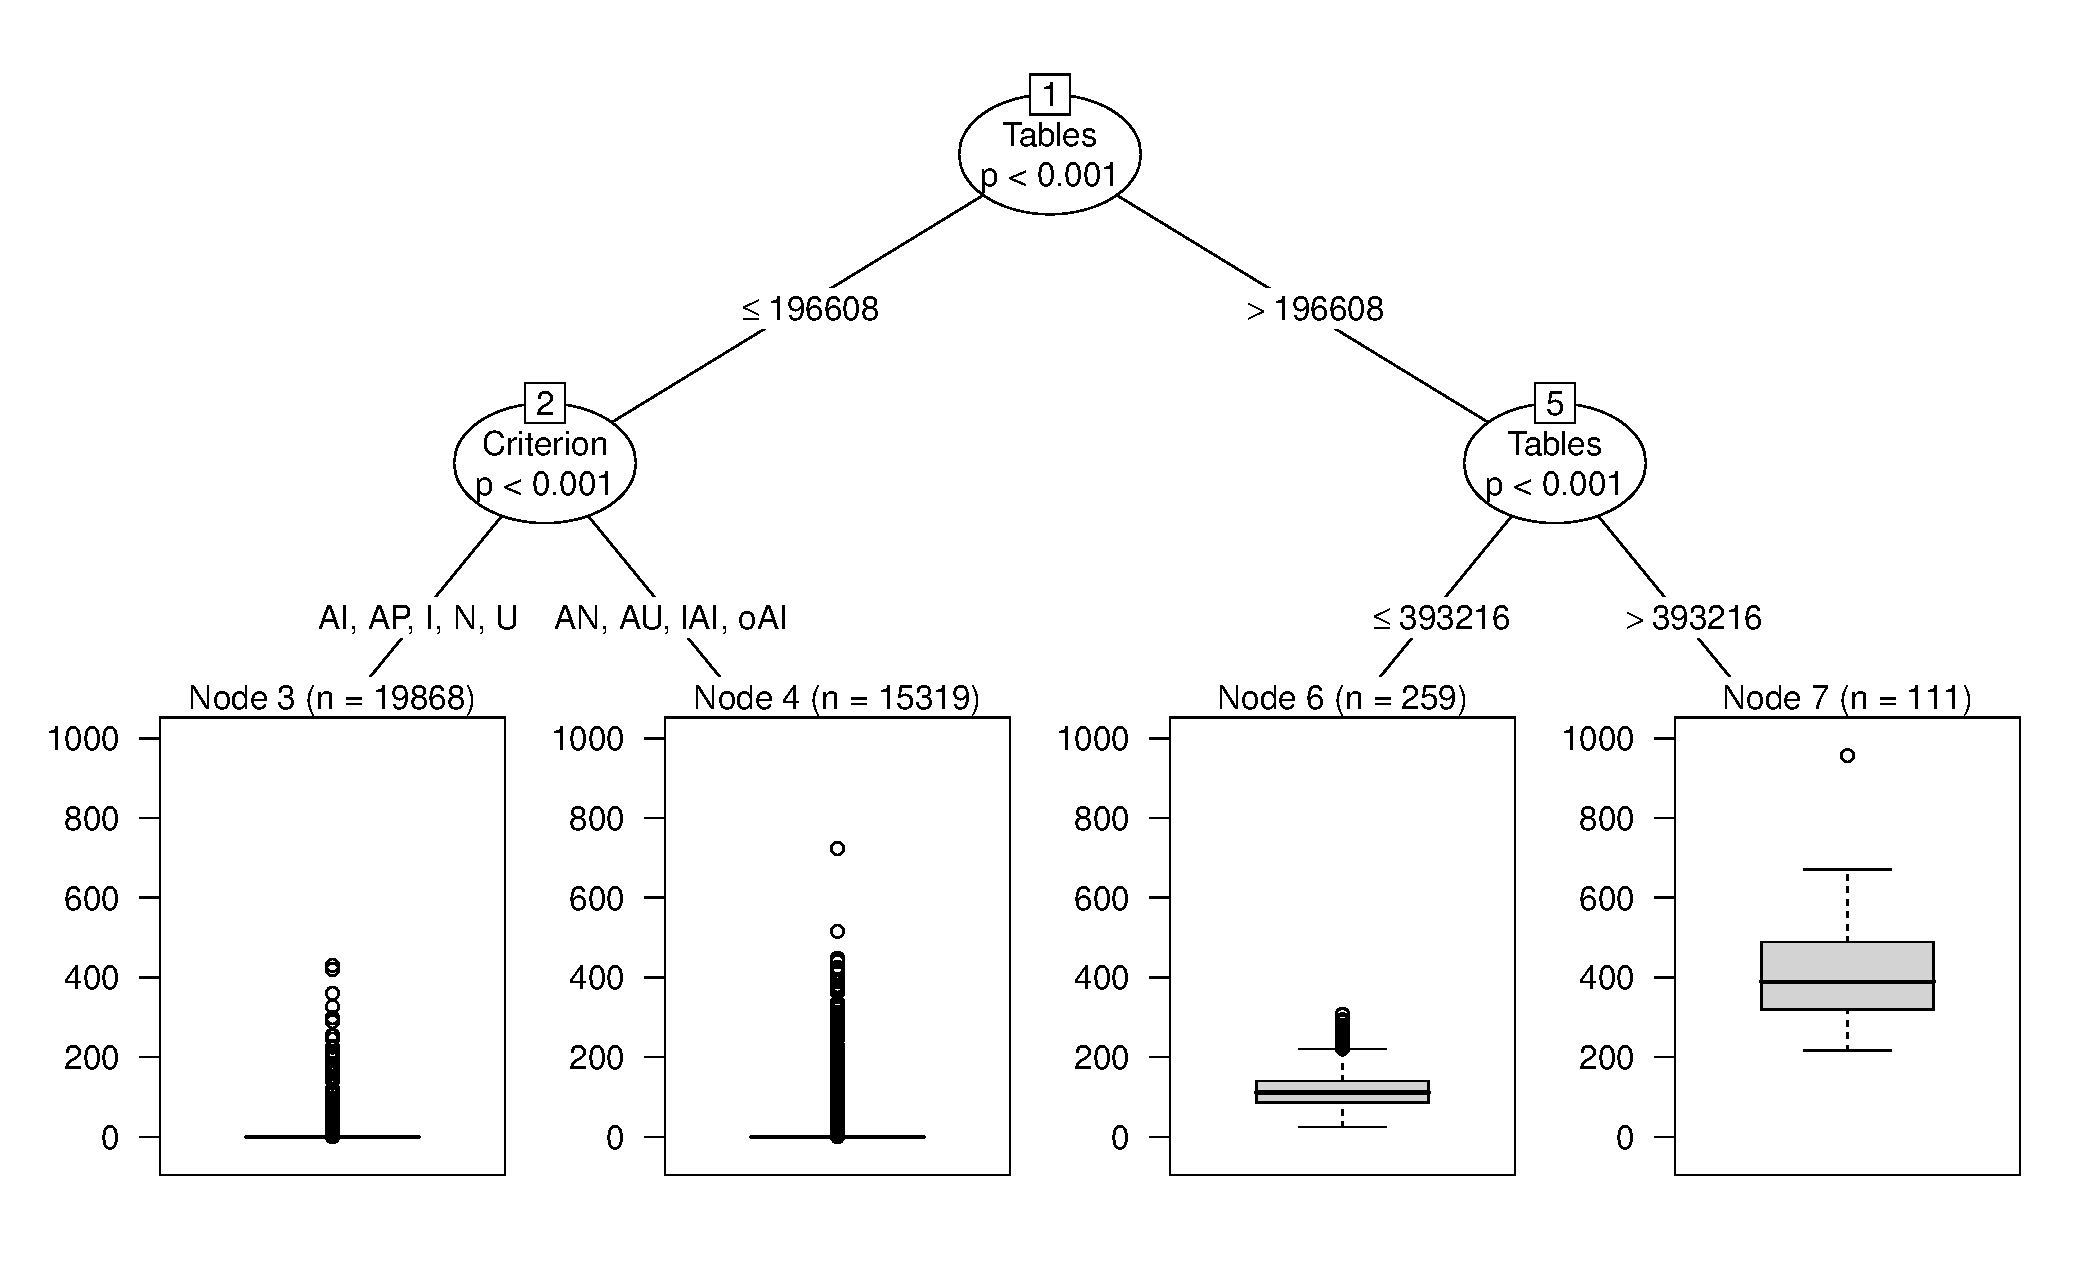
\includegraphics[width=.75\linewidth]{../diagrams/AllTree.pdf}
  \caption{Regression tree using all variables to predict runtime in
  minutes. \vspace{-.15in}}
  \label{fig:atree}
  \vspace{-.15in} 
\end{figure*}

\begin{figure*}
\centering
  \centering
  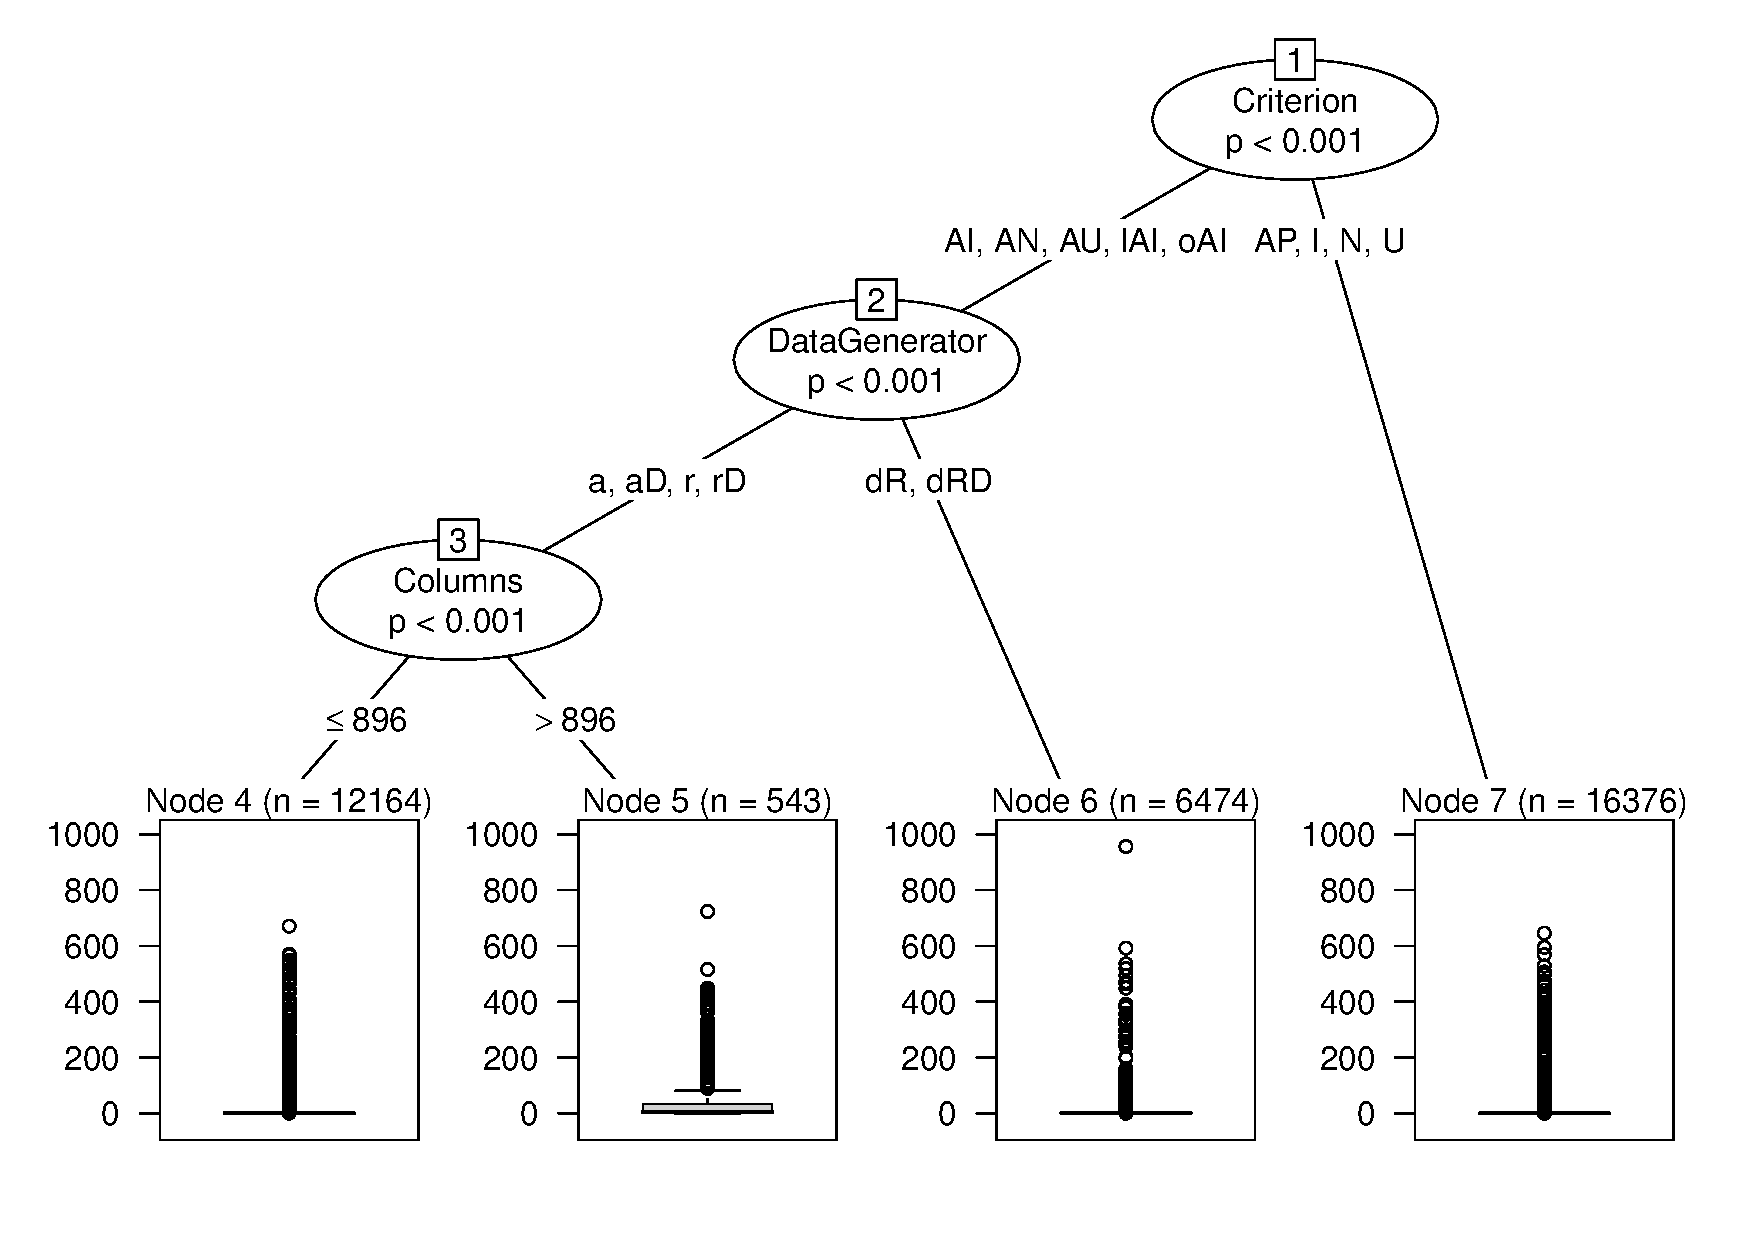
\includegraphics[width=.75\linewidth]{../diagrams/NoTableCtreesd.pdf}
  \caption{Regression tree predicting runtime excluding Tables.\vspace{-.15in}}
  \label{fig:ttree}
  \vspace{-.15in} 
\end{figure*}


\begin{figure}
\centering
  \centering
  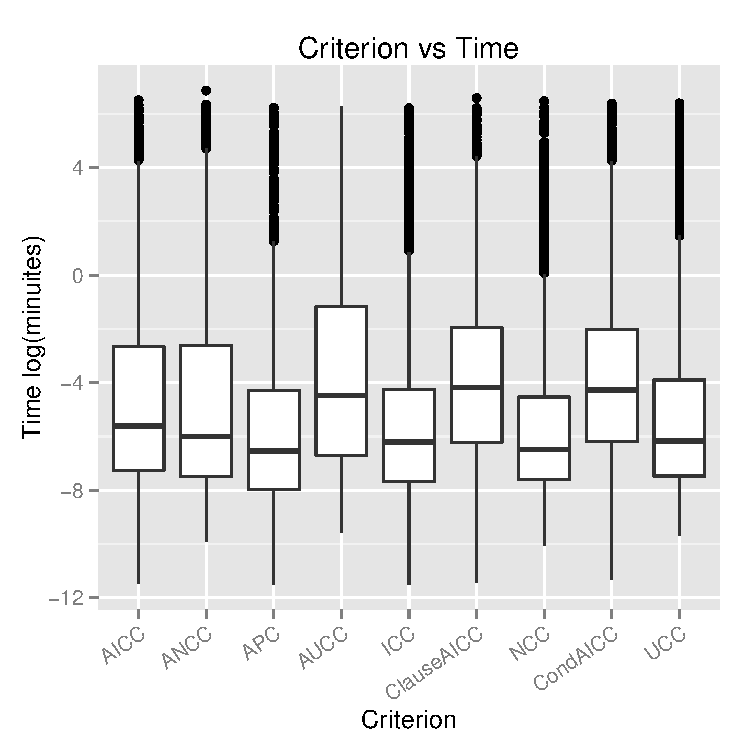
\includegraphics[width=1\linewidth]{../diagrams/CriterionvsTime.pdf}
  \caption{Coverage criterion versus runtime in minutes.\vspace{-.15in}}
  \label{fig:crites}
  \vspace{-.15in} 
\end{figure}

\begin{figure}
\centering
  \centering
  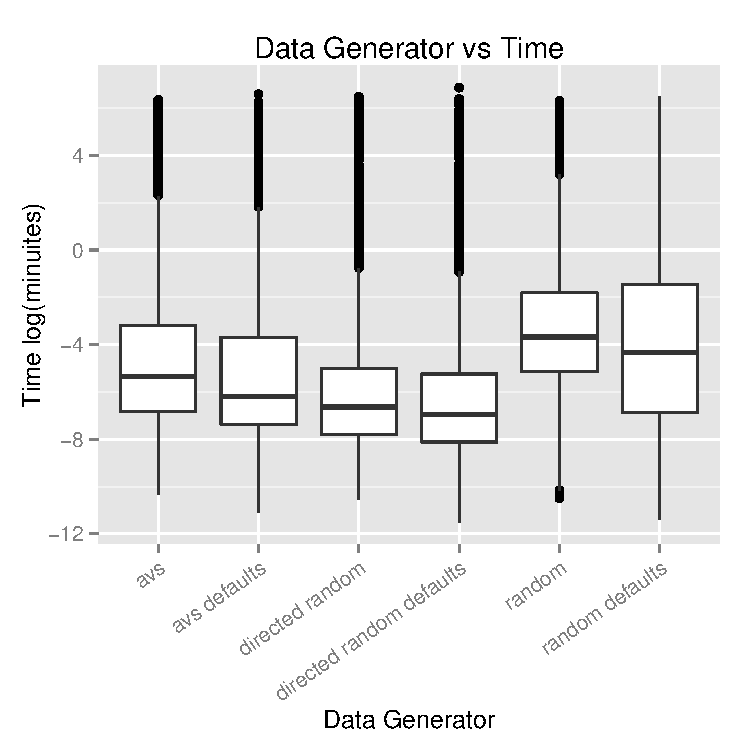
\includegraphics[width=1\linewidth]{../diagrams/DataGeneratorvsTime.pdf}
  \caption{Data generator versus runtime in minutes.\vspace{-.15in}}
  \label{fig:datas}
  \vspace{-.15in} 
\end{figure}


\begin{table*}[h]
\begin{tabular}{llllllllll}
           & APC      & ANCC     & CondAICC & NCC      & AUCC     & AICC     & ClauseAICC & ICC      & UCC   \\ 
APC        & NA       & 0.425    & 0.337    & 0.484    & 0.334    & 0.413    & 0.329      & 0.481    & 0.449 \\
ANCC       & 2.20E-16 & NA       & 0.407    & 0.561    & 0.405    & 0.484    & 0.399      & 0.554    & 0.526 \\
CondAICC   & 2.20E-16 & 2.20E-16 & NA       & 0.671    & 0.503    & 0.581    & 0.492      & 0.656    & 0.634 \\
NCC        & 1.20E-02 & 2.20E-16 & 2.20E-16 & NA       & 0.335    & 0.417    & 0.322      & 0.491    & 0.461 \\
AUCC       & 2.20E-16 & 2.20E-16 & 6.92E-01 & 2.20E-16 & NA       & 0.577    & 0.490      & 0.651    & 0.628 \\
AICC       & 2.20E-16 & 1.70E-02 & 2.20E-16 & 2.20E-16 & 2.20E-16 & NA       & 0.412      & 0.571    & 0.547 \\
ClauseAICC & 2.20E-16 & 2.20E-16 & 2.72E-01 & 2.20E-16 & 1.40E-01 & 2.20E-16 & NA         & 0.662    & 0.641 \\
ICC        & 4.00E-03 & 2.20E-16 & 2.20E-16 & 1.83E-01 & 2.20E-16 & 2.20E-16 & 2.20E-16   & NA       & 0.472 \\
UCC        & 9.30E-16 & 3.83E-05 & 2.20E-16 & 7.36E-10 & 2.20E-16 & 5.73E-13 & 2.20E-16   & 9.29E-06 & NA    \\ 
\end{tabular}
\caption{For each pair of coverage criterions, lower left shows Wilcox
Rank Sum Test, upper right shows $\hat{A}_{12}$.}
\label{tab:crites}
\end{table*}


\begin{table*}[h]
\begin{tabular}{lllllll}
                         & Random   & Random Defaults & Directed Random & Directed Random Defaults & AVM      & AVM Defaults \\
Random                   & NA       & 0.538           & 0.740           & 0.789                    & 0.627    & 0.680        \\
Random Defaults          & 6.59E-13 & NA              & 0.673           & 0.701                    & 0.564    & 0.617        \\
Directed Random          & 2.20E-16 & 2.20E-16        & NA              & 0.543                    & 0.360    & 0.435        \\
Directed Random Defaults & 2.20E-16 & 2.20E-16        & 9.74E-16        & NA                       & 0.328    & 0.395        \\
AVM                      & 2.20E-16 & 2.20E-16        & 2.20E-16        & 2.20E-16                 & NA       & 0.572        \\
AVM Defaults             & 2.20E-16 & 2.20E-16        & 2.20E-16        & 2.20E-16                 & 2.20E-16 & NA          
\end{tabular}
\caption{For each pair of Data Generators, lower left shows Wilcox Rank
Sum Test, upper right shows $\hat{A}_{12}$.}
\label{tab:datas}
\end{table*}


\subsection*{Threats to Validity}

Our technique for doubling the number of check constraints on the schema
is simply to duplicate the existing check constraints. It is possible
that \textit{SchemaAnalyst} does less work processing these copied check
constraints than it would given unique check constraints. However,
doubling the check constraints in this way is an easy to implement,
semantically significant way of evaluating \textit{SchemaAnalyst}.

Additionally, since worst-case time is only apparent for large $n$, 
it is possible that the experiment terminated too quickly.  To guard 
against this problem, Algorithms~\ref{alg:convergence} and~\ref{alg:tuning}
were tested on various other algorithms with known worst-case complexities, and 
found to be reliable.
